\providecommand{\setflag}{\newif \ifwhole \wholefalse}
\setflag
\ifwhole\else

% Typography and geometry ----------------------------------------------------
\documentclass[letterpaper]{scrbook}
\usepackage[inner=3cm,top=2.5cm,outer=3.5cm]{geometry}

\renewcommand\familydefault{bch}
\usepackage[utf8]{inputenc}
\usepackage{microtype}
\usepackage[small]{caption}
\usepackage[small]{titlesec}
\raggedbottom

% Graphics -------------------------------------------------------------------
\usepackage[pdftex]{graphicx}
\graphicspath{{_include/}}
\DeclareGraphicsExtensions{.png,.pdf}

% Code formatting ------------------------------------------------------------
\usepackage{fancyvrb}
\usepackage{courier}
\usepackage{listings}
\usepackage{color}
\usepackage{alltt}


\definecolor{comment}{rgb}{0.60, 0.60, 0.53}
\definecolor{background}{rgb}{0.97, 0.97, 1.00}
\definecolor{string}{rgb}{0.863, 0.066, 0.266}
\definecolor{number}{rgb}{0.0, 0.6, 0.6}
\definecolor{variable}{rgb}{0.00, 0.52, 0.70}
\lstset{
  basicstyle=\ttfamily,
  keywordstyle=\bfseries, 
  identifierstyle=,  
  commentstyle=\color{comment} \emph,
  stringstyle=\color{string},
  showstringspaces=false,
  columns = fullflexible,
  backgroundcolor=\color{background},
  mathescape = true,
  escapeinside=&&,
  fancyvrb
}
\newcommand{\code}[1]{\lstinline!#1!}
\newcommand{\f}[1]{\lstinline!#1()!}



% Links ----------------------------------------------------------------------

\usepackage{hyperref}
\definecolor{slateblue}{rgb}{0.07,0.07,0.488}
\hypersetup{colorlinks=true,linkcolor=slateblue,anchorcolor=slateblue,citecolor=slateblue,filecolor=slateblue,urlcolor=slateblue,bookmarksnumbered=true,pdfview=FitB}
\usepackage{url}

% Tables ---------------------------------------------------------------------
\usepackage{longtable}
\usepackage{booktabs}

% Miscellaneous --------------------------------------------------------------
\usepackage{pdfsync}
\usepackage{appendix}

\usepackage[round,sort&compress,sectionbib]{natbib}
\bibliographystyle{plainnat}


\title{ggplot2}
\author{Hadley Wickham}

\begin{document}
\fi


% qplot chapter suggestions:
% 
% * exercises - see plot and then try and create on your own
% * wall chart of different plot types
% * more error bar and ribbon examples
% * table of options

% SET_DEFAULTS
%   GG-WIDTH: 4 GG-HEIGHT: 2.4
%   TEX-WIDTH: 0.5\linewidth
%   INLINE: FALSE
%   CACHE: TRUE
% 

% END

\chapter{Getting started with qplot}
\label{cha:qplot}

\section{Introduction} 

In this chapter, you will learn to make a wide variety of plots with your first \ggplot function, \f{qplot}, short for {\bf q}uick plot. \code{qplot} makes it easy to produce complex plots, often requiring several lines of code using other plotting systems, in one line. \f{qplot} can do this because it's based on the grammar of graphics, which allows you to create a simple, yet expressive, description of the plot.  In later chapters you'll learn to use all of the expressive power of the grammar, but here we'll start simple so you can work your way up.  You will also start to learn some of the \ggplot terminology that will be used throughout the book.

{\tt qplot} has been designed to be very similar to {\tt plot}, which should make it easy if you're already familiar with plotting in R.  Remember, during an R session you can get a summary of all the arguments to {\tt qplot} with R help, {\tt ?qplot}.

In this chapter you'll learn:

\begin{itemize}
  \item The basic use of {\tt qplot}---If you're already familiar with {\tt plot}, this will be particularly easy, \secref{sec:basic_use}.
  \item How to map variables to aesthetic attributes, like colour, size and shape, \secref{sec:aesthetic_attributes}.
  \item How to create many different types of plots by specifying different geoms, and how to combine multiple types in a single plot,  \secref{sec:plot_geoms}.
  \item The use of faceting, also known as trellising or conditioning, to break apart subsets of your data, \secref{sec:qplot-faceting}.
  \item How to tune the appearance of the plot by specifying some basic options, \secref{sec:other_options}.
  \item A few important differences between \f{plot} and \f{qplot}, \secref{sec:plot_diffs}.
\end{itemize}

\section{Datasets}\label{sec:data_sets}

In this chapter we'll just use one data source, so you can get familiar with the plotting details rather than having to familiarise yourself with different datasets. The {\tt diamonds} dataset consists of prices and quality information about 54,000 diamonds, and is included in the \ggplot package. The data contains the four C's of diamond quality, carat, cut, colour and clarity; and five physical measurements, depth, table, x, y and z, as described in Figure~\ref{fig:diamond-dim}.  The first few rows of the data are shown in Table~\ref{tab:diamonds}.

\begin{table}[ht]
\begin{center}
\begin{tabular}{lrrrrrrrrrr}
  \toprule
  carat & cut & color & clarity & depth & table & price & x & y & z \\
  \midrule
  0.2 & Ideal & E & SI2 & 61.5 & 55.0 & 326 & 3.95 & 3.98 & 2.43 \\
  0.2 & Premium & E & SI1 & 59.8 & 61.0 & 326 & 3.89 & 3.84 & 2.31 \\
  0.2 & Good & E & VS1 & 56.9 & 65.0 & 327 & 4.05 & 4.07 & 2.31 \\
  0.3 & Premium & I & VS2 & 62.4 & 58.0 & 334 & 4.20 & 4.23 & 2.63 \\
  0.3 & Good & J & SI2 & 63.3 & 58.0 & 335 & 4.34 & 4.35 & 2.75 \\
  0.2 & Very Good & J & VVS2 & 62.8 & 57.0 & 336 & 3.94 & 3.96 & 2.48 \\
  \bottomrule
\end{tabular}
\caption{{\tt diamonds} dataset.  The variables depth, table, x, y and z refer to the dimensions of the diamond as shown in Figure~\ref{fig:diamond-dim}}
\label{tab:diamonds}
\end{center}
\end{table}

\begin{figure}[htbp]
  \centering
    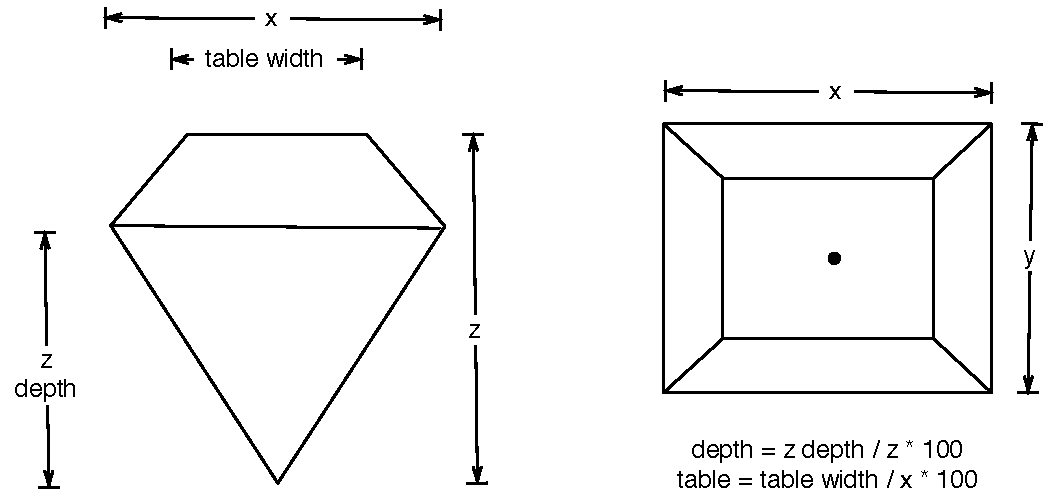
\includegraphics[width=0.8\linewidth]{diamond-dimensions}
  \caption{How the variables x, y, z, table and depth are measured.}
  \label{fig:diamond-dim}
\end{figure}

The dataset has not been well cleaned, so as well as demonstrating interesting relationships about diamonds, it also demonstrates some data quality problems. We'll also use another dataset, {\tt dsmall}, which is a random sample of 100 diamonds. We'll use this data for plots that are more appropriate for smaller datasets. 

% INTERWEAVE
% 
% set.seed(1410) # Make the sample reproducible
% dsmall <- diamonds[sample(nrow(diamonds), 100), ]
\input{_include/1b3ba81ba23901fc35089ffdc0895538.tex}
% END

\section{Basic use}
\label{sec:basic_use}

As with  {\tt plot}, the first two arguments to \f{qplot} are {\tt x} and {\tt y}, giving the x- and y-coordinates for the objects on the plot. There is also an optional {\tt data} argument.  If this is specified, \f{qplot} will look inside that data frame before looking for objects in your workspace.  Using the \code{data} argument is recommended: it's a good idea to keep related data in a single data frame.  If you don't specify one, \f{qplot} will try to build one up for you and may look in the wrong place.

Here is a simple example of the use of \f{qplot}.  It produces a scatterplot showing the relationship between the price and carats (weight) of a diamond. 

% INTERWEAVE
%   FILETYPE: png
% 
% qplot(carat, price, data = diamonds)
\input{_include/eaaf8d759dac450315433a2e0d229cba.tex}
% END

The plot shows a strong correlation with notable outliers and some interesting vertical striation.  The relationship looks exponential, though, so the first thing we'd like to do is to transform the variables.  Because \f{qplot} accepts functions of variables as arguments, we plot log(price) vs.\ log(carat):

% INTERWEAVE
%   FILETYPE: png
% 
% qplot(log(carat), log(price), data = diamonds)
\input{_include/a08a0ecfbca79add95ee81fbcc588042.tex}
% END

\noindent The relationship now looks linear.  With this much overplotting, though, we need to be cautious about drawing firm conclusions.

Arguments can also be combinations of existing variables, so, if we are curious about the relationship between the volume of the diamond (approximated by $x \times y \times z$) and its weight, we could do the following:

% INTERWEAVE
%   FILETYPE: png
% 
% qplot(carat, x * y * z, data = diamonds)
\input{_include/68e6557164a5bee939594c9a35d24e2a.tex}
% END

We would expect the density (weight/volume) of diamonds to be constant, and so see a linear relationship between volume and weight. The majority of diamonds do seem to fall along a line, but there are some large outliers.

\section{Colour, size, shape and other aesthetic attributes}
\label{sec:aesthetic_attributes}

The first big difference when using {\tt qplot} instead of {\tt plot} comes when you want to assign colours---or sizes or shapes---to the points on your plot.  With {\tt plot}, it's your responsibility to convert a categorical variable in your data (e.g., ``apples'', ``bananas'', ``pears'') into something that {\tt plot} knows how to use (e.g., ``red'', ``yellow'', ``green'').  {\tt qplot} can do this for you automatically, and it will automatically provide a legend that maps the displayed attributes to the data values.  This makes it easy to include additional data on the plot.  

In the next example, we augment the plot of carat and price with information about diamond colour and cut.  The results are shown in Figure~\ref{fig:qplot-aesthetics}.

% FIGLISTING
%   LABEL: qplot-aesthetics
%   CAPTION: Mapping point colour to diamond colour (left), and point shape 
%   to cut quality (right).
% 
% qplot(carat, price, data = dsmall, colour = color)
% qplot(carat, price, data = dsmall, shape = cut)
\input{_include/b177b6c55087925675ed42d698509be7.tex}
% END

Colour, size and shape are all examples of aesthetic attributes, visual properties that affect the way observations are displayed. For every aesthetic attribute, there is a function, called a \emph{scale}, which maps data values to valid values for that aesthetic. It is this scale that controls the appearance of the points and associated legend. For example, in the above plots, the colour scale maps J to purple and F to green. (Note that while I use British spelling throughout this book, the software also accepts American spellings.)

You can also manually set the aesthetics using \f{I}, e.g., \code{colour = I("red")} or \code{size = I(2)}.  This is not the same as mapping and is explained in more detail in Section~\ref{sub:setting-mapping}.  For large datasets, like the diamonds data, semi-transparent points are often useful to alleviate some of the overplotting.  To make a semi-transparent colour you can use the alpha aesthetic, which takes a value between 0 (completely transparent) and 1 (complete opaque).  It's often useful to specify the transparency as a fraction, e.g., \code{1/10} or \code{1/20}, as the denominator specifies the number of points that must overplot to get a completely opaque colour. 

% FIGLISTING
%   FILETYPE: png
%   LABEL: qplot-set
%   CAPTION: Reducing the alpha value from 1/10 (left) to 1/100 (middle) to
%   1/200 (right) makes it possible to see where the bulk of the points lie.
%   TEX-WIDTH: 0.33\linewidth GG-WIDTH: 4 GG-HEIGHT: 4
% 
% qplot(carat, price, data = diamonds, alpha = I(1/10))
% qplot(carat, price, data = diamonds, alpha = I(1/100))
% qplot(carat, price, data = diamonds, alpha = I(1/200))
\input{_include/b82f972884dd3198b67581be66834d90.tex}
% END

Different types of aesthetic attributes work better with different types of variables. For example, colour and shape work well with categorical variables, while size works better with continuous variables. The amount of data also makes a difference: if there is a lot of data, like in the plots above, it can be hard to distinguish the different groups. An alternative solution is to use faceting, which will be introduced in Section~\ref{sec:qplot-faceting}.

\section{Plot geoms}\label{sec:plot_geoms}

{\tt qplot} is not limited to scatterplots, but can produce almost any kind of plot by varying the {\tt geom}. Geom, short for geometric object, describes the type of object that is used to display the data. Some geoms have an associated statistical transformation, for example, a histogram is a binning statistic plus a bar geom. These different components are described in the next chapter. Here we'll introduce the most common and useful geoms, organised by the dimensionality of data that they work with. The following geoms enable you to investigate two-dimensional relationships:

\begin{itemize}

  \item {\tt geom = "point"} draws points to produce a scatterplot. This is the default when you supply both \code{x} and \code{y} arguments to \f{qplot}.

  \item {\tt geom = "smooth"} fits a smoother to the data and displays the smooth and its standard error, \secref{sub:smooth}.

  \item {\tt geom = "boxplot"} produces a box-and-whisker plot to summarise the distribution of a set of points, \secref{sub:boxplot}.

  \item {\tt geom = "path"} and {\tt geom = "line"} draw lines between the data points.  Traditionally these are used to explore relationships between time and another variable, but lines may be used to join observations connected in some other way.  A line plot is constrained to produce lines that travel from left to right, while paths can go in any direction,  \secref{sub:line}.
\end{itemize}

\noindent For 1d distributions, your choice of geoms is guided by the variable type:

\begin{itemize}
  \item For continuous variables, {\tt geom = "histogram"} draws a histogram, {\tt geom = "freqpoly"} a frequency polygon, and {\tt geom = "density"} creates a density plot, \secref{sub:distribution}.  The histogram geom is the default when you only supply an \code{x} value to \f{qplot}.

  \item For discrete variables, {\tt geom = "bar"} makes a bar chart, \secref{sub:bar}.

\end{itemize}


\subsection{Adding a smoother to a plot}\label{sub:smooth}

If you have a scatterplot with many data points, it can be hard to see exactly what trend is shown by the data. In this case you may want to add a smoothed line to the plot. This is easily done using the {\tt smooth} geom as shown in Figure~\ref{fig:qplot-smooth}. Notice that we have combined multiple geoms by supplying a vector of geom names created with \f{c}.  The geoms will be overlaid in the order in which they appear.  

% FIGLISTING
%   FILETYPE: png
%   LABEL: qplot-smooth
%   CAPTION: Smooth curves add to scatterplots of carat vs.\ price. The
%   dsmall dataset (left) and the full dataset (right).
% 
% qplot(carat, price, data = dsmall, geom = c("point", "smooth"))
% qplot(carat, price, data = diamonds, geom = c("point", "smooth"))
\input{_include/f39705aa35a5d684159fbb3cfb0987d1.tex}
% END

Despite overplotting, our impression of an exponential relationship between price and carat was correct. There are few diamonds bigger than three carats, and our uncertainty in the form of the relationship increases as illustrated by the point-wise confidence interval shown in grey. If you want to turn the confidence interval off, use {\tt se = FALSE}. 

There are many different smoothers you can choose between by using the {\tt method} argument:

\begin{itemize}
  \item {\tt method = "loess"}, the default for small n, uses a smooth local regression.  More details about the algorithm used can be found in {\tt ?loess}.  The wiggliness of the line is controlled by the \code{span} parameter, which ranges from 0 (exceedingly wiggly) to 1 (not so wiggly), as shown in Figure~\ref{fig:smooth-loess}.  
  
  % FIGLISTING
  %   FILETYPE: png
  %   LABEL: smooth-loess
  %   CAPTION: The effect of the span parameter.  (Left) \code{span = 0.2}, 
  %   and (right) \code{span = 1}.
  % 
  % qplot(carat, price, data = dsmall, geom = c("point", "smooth"), 
  %   span = 0.2)
  % qplot(carat, price, data = dsmall, geom = c("point", "smooth"), 
  %   span = 1)
  \input{_include/47fbf50afac737a07ef5db1e078645a1.tex}  
  % END
  
  \noindent Loess does not work well for large datasets (it's $O(n^2)$ in memory), and so an alternative smoothing algorithm is used when $n$ is greater than 1,000.

  \item You could also load the {\tt mgcv} library and use {\tt method = "gam", formula = y $\sim$ s(x)} to fit a generalised additive model. This is similar to using a spline with {\tt lm}, but the degree of smoothness is estimated from the data.  For large data, use the formula {\tt y \verb|~| s(x, bs = "cs")}.  This is used by default when there are more than 1,000 points.

  % FIGLISTING
  %   FILETYPE: png
  %   LABEL: smooth-gam
  %   CAPTION: The effect of the formula parameter, using a generalised
  %   additive model as a smoother.  (Left) \code{formula = y ~ s(x)}, the
  %   default; (right) \code{formula = y ~ s(x, bs = "cs")}.
  % 
  % library(mgcv)
  % qplot(carat, price, data = dsmall, geom = c("point", "smooth"), 
  %   method = "gam", formula = y ~ s(x))
  % qplot(carat, price, data = dsmall, geom = c("point", "smooth"), 
  %   method = "gam", formula = y ~ s(x, bs = "cs"))
  \input{_include/1a71bb8d30191d3d57cf61b71353b15a.tex}  
  % END

  \item {\tt method = "lm"} fits a linear model.  The default will fit a straight line to your data, or you can specify {\tt formula = y \verb|~| poly(x, 2)} to specify a degree 2 polynomial, or better, load the {\tt splines} package and use a natural spline: {\tt formula = y \verb|~| ns(x, 2)}. The second parameter is the degrees of freedom: a higher number will create a wigglier curve. You are free to specify any formula involving $x$ and $y$.  Figure~\ref{fig:smooth-lm} shows two examples created with the following code.  

  % FIGLISTING
  %   FILETYPE: png
  %   LABEL: smooth-lm
  %   CAPTION: The effect of the formula parameter, using a linear model
  %   as a smoother.  (Left) \code{formula = y ~ x}, the default; (right)
  %   \code{formula = y ~ ns(x, 5)}.
  % 
  % library(splines)
  % qplot(carat, price, data = dsmall, geom = c("point", "smooth"), 
  %   method = "lm")
  % qplot(carat, price, data = dsmall, geom = c("point", "smooth"), 
  %   method = "lm", formula = y ~ ns(x,5))
  \input{_include/358579be390b704635d9bbb92f3d1ffc.tex}  
  % END

  \item {\tt method = "rlm"} works like {\tt lm}, but uses a robust fitting algorithm so that outliers don't affect the fit as much.  It's part of the {\tt MASS} package, so remember to load that first.

\end{itemize}

\subsection{Boxplots and jittered points}
\label{sub:boxplot}

When a set of data includes a categorical variable and one or more continuous variables, you will probably be interested to know how the values of the continuous variables vary with the levels of the categorical variable.  Box-plots and jittered points offer two ways to do this.  Figure~\ref{fig:jitter-boxplot} explores how the distribution of price per carat varies with the colour of the diamond using jittering ({\tt geom = "jitter"}, left) and box-and-whisker plots ({\tt geom = "boxplot"}, right).

% FIGURE
%   LABEL: jitter-boxplot
%   FILETYPE: png
%   CAPTION: Using jittering (left) and boxplots (right) to investigate
%   the distribution of price per carat, conditional on colour.  As the colour
%   improves (from left to right) the spread of values decreases, but there
%   is little change in the centre of the distribution.
% 
% qplot(color, price / carat, data = diamonds, geom = "jitter")
% qplot(color, price / carat, data = diamonds, geom = "boxplot")
\input{_include/09c93ac71800ac3ba85d3ec375a707f6.tex}
% END

Each method has its strengths and weaknesses. Boxplots summarise the bulk of the distribution with only five numbers, while jittered plots show every point but can suffer from overplotting. In the example here, both plots show the dependency of the spread of price per carat on diamond colour, but the boxplots are more informative, indicating that there is very little change in the median and adjacent quartiles.

The overplotting seen in the plot of jittered values can be alleviated somewhat by using semi-transparent points using the {\tt alpha} argument. Figure~\ref{fig:jitter-alpha} illustrates three different levels of transparency, which make it easier to see where the bulk of the points lie.  The plots are produced with the following code.

% FIGLISTING
%   LABEL: jitter-alpha
%   FILETYPE: png
%   CAPTION: Varying the alpha level.  From left to right: $1/5$, $1/50$,
%   $1/200$.  As the opacity decreases we begin to see where the bulk of the
%   data lies.  However, the boxplot still does much better.
%   GG-WIDTH: 3 GG-HEIGHT: 3 TEX-WIDTH: 0.33\linewidth
% 
% qplot(color, price / carat, data = diamonds, geom = "jitter",
%  alpha = I(1 / 5))
% qplot(color, price / carat, data = diamonds, geom = "jitter",
%  alpha = I(1 / 50))
% qplot(color, price / carat, data = diamonds, geom = "jitter",
%  alpha = I(1 / 200))
\input{_include/1030d1a724f00e8e3a37613eaa0ad665.tex}
% END

This technique can't show the positions of the quantiles as well as a boxplot can, but it may reveal other features of the distribution that a boxplot cannot.

For jittered points, {\tt qplot} offers the same control over aesthetics as it does for a normal scatterplot: {\tt size}, {\tt colour} and {\tt shape}. For boxplots you can control the outline \code{colour}, the internal \code{fill} colour and the \code{size} of the lines.

Another way to look at conditional distributions is to use faceting to plot a separate histogram or density plot for each value of the categorical variable.  This is demonstrated in Section~\ref{sec:qplot-faceting}.

\subsection{Histogram and density plots}\label{sub:distribution}

Histogram and density plots show the distribution of a single variable.  They provide more information about the distribution of a single group than boxplots do, but it is harder to compare many groups (although we will look at one way to do so).  Figure~\ref{fig:dist} shows the distribution of carats with a histogram and a density plot.

% FIGLISTING
%   LABEL: dist
%   GG-WIDTH: 4 GG-HEIGHT: 3
%   CAPTION: Displaying the distribution of diamonds.  (Left) 
%   \code{geom = "histogram"} and (right) \code{geom = "density"}.
% 
% qplot(carat, data = diamonds, geom = "histogram")
% qplot(carat, data = diamonds, geom = "density")
\input{_include/154eed52321404cbf12fbb131e43239d.tex}
% END

For the density plot, the {\tt adjust} argument controls the degree of smoothness (high values of {\tt adjust} produce smoother plots). For the histogram, the {\tt binwidth} argument controls the amount of smoothing by setting the bin size.  (Break points can also be specified explicitly, using the {\tt breaks} argument.) It is {\bf very important} to experiment with the level of smoothing.  With a histogram you should try many bin widths: You may find that gross features of the data show up well at a large bin width, while finer features require a very narrow width.

In Figure~\ref{fig:hist-binwidth}, we experiment with three values of {\tt binwidth}: 1.0, 0.1 and 0.01.  It is only in the plot with the smallest bin width (right) that we see the striations we noted in an earlier scatterplot, most at ``nice'' numbers of carats. The full code is:

% FIGLISTING
%   LABEL: hist-binwidth
%   TEX-WIDTH: 0.33\linewidth
%   GG-WIDTH: 4 GG-HEIGHT: 3
%   CAPTION:  Varying the bin width on a histogram of carat reveals 
%   interesting patterns.  Binwidths from left to right: 1, 0.1 and 0.01 
%   carats. Only diamonds between 0 and 3 carats shown. 
% 
% qplot(carat, data = diamonds, geom = "histogram", binwidth = 1, 
%   xlim = c(0,3))
% qplot(carat, data = diamonds, geom = "histogram", binwidth = 0.1,
%   xlim = c(0,3))
% qplot(carat, data = diamonds, geom = "histogram", binwidth = 0.01,
%   xlim = c(0,3))
\input{_include/cd83a8e53e1ab8f6dea025e37aa9f20f.tex}
% END

To compare the distributions of different subgroups, just add an aesthetic mapping, as in the following code.

% FIGLISTING
%   GG-WIDTH: 4 GG-HEIGHT: 3
%   LABEL: dist-fill
%   CAPTION: Mapping a categorical variable to an aesthetic will automatically
%   split up the geom by that variable.  (Left) Density plots are overlaid
%   and (right) histograms are stacked.
% 
% qplot(carat, data = diamonds, geom = "density", colour = color)
% qplot(carat, data = diamonds, geom = "histogram", fill = color)
\input{_include/518c885d41a273ee50d0346bdab9e6ff.tex}
% END

\noindent Mapping a categorical variable to an aesthetic will automatically split up the geom by that variable, so these commands instruct \f{qplot} to draw a density plot and histogram for each level of diamond colour. The results are shown in Figure~\ref{fig:dist-fill}.  

The density plot is more appealing at first because it seems easy to read and compare the various curves. However, it is more difficult to understand exactly what a density plot is showing.  In addition, the density plot makes some assumptions that may not be true for our data; i.e., that it is unbounded, continuous and smooth.

\subsection{Bar charts}
\label{sub:bar}

The discrete analogue of histogram is the bar chart,~\code{geom = "bar"}. The bar geom counts the number of instances of each class so that you don't need to tabulate your values beforehand, as with \code{barchart} in base R. If the data has already been tabulated or if you'd like to tabulate class members in some other way, such as by summing up a continuous variable, you can use the \code{weight} geom. This is illustrated in Figure~\ref{fig:dist-bar}. The first plot is a simple bar chart of diamond colour, and the second is a bar chart of diamond colour weighted by carat.

% FIGLISTING
%   LABEL: dist-bar
%   GG-WIDTH: 4 GG-HEIGHT: 2.4
%   CAPTION: Bar charts of diamond colour.  The left plot shows counts and the 
%   right plot is weighted by \code{weight = carat} to show the total weight
%   of diamonds of each colour.
% 
% qplot(color, data = diamonds, geom = "bar")
% qplot(color, data = diamonds, geom = "bar", weight = carat) +
%   scale_y_continuous("carat")
\input{_include/6c980956a0a79e34fc3a263f462ddce5.tex}
% END

\subsection{Time series with line and path plots}
\label{sub:line}

Line and path plots are typically used for time series data.  Line plots join the points from left to right, while path plots join them in the order that they appear in the dataset (a line plot is just a path plot of the data sorted by x value).  Line plots usually have time on the x-axis, showing how a single variable has changed over time.  Path plots show how two variables have simultaneously changed over time, with time encoded in the way that the points are joined together.

Because there is no time variable in the diamonds data, we use the {\tt economics} dataset, which contains economic data on the US measured over the last 40 years. Figure~\ref{fig:line-employment} shows two plots of unemployment over time, both produced using {\tt geom = "line"}. The first shows an unemployment rate and the second shows the median number of weeks unemployed. We can already see some differences in these two variables, particularly in the last peak, where the unemployment percentage is lower than it was in the preceding peaks, but the length of unemployment is high.

% FIGLISTING
%  LABEL: line-employment
%  GG-WIDTH: 4 GG-HEIGHT: 2.4
%  CAPTION: Two time series measuring amount of unemployment.  (Left) 
%   Percent of population that is unemployed and (right) median
%   number of weeks unemployed.  Plots created with {\tt geom="line"}.
% 
% qplot(date, unemploy / pop, data = economics, geom = "line")
% qplot(date, uempmed, data = economics, geom = "line")
\input{_include/a0f78f7d9c4b90d93280ab0aefb83bfc.tex}
% END

To examine this relationship in greater detail, we would like to draw both time series on the same plot. We could draw a scatterplot of unemployment rate vs.\ length of unemployment, but then we could no longer see the evolution over time. The solution is to join points adjacent in time with line segments, forming a \emph{path} plot.

Below we plot unemployment rate vs.\ length of unemployment and join the individual observations with a path. Because of the many line crossings, the direction in which time flows isn't easy to see in the first plot. In the second plot, we apply the {\tt colour} aesthetic to the line to make it easier to see the direction of time.

% FIGLISTING
%   GG-WIDTH: 4 GG-HEIGHT: 2.4
%   LABEL: path-employ
%   CAPTION: Path plots illustrating the relationship between percent of 
%   people unemployed and median length of unemployment.  (Left) Scatterplot
%   with overlaid path.  (Right) Pure path plot coloured by year.
% 
% year <- function(x) as.POSIXlt(x)$year + 1900
% qplot(unemploy / pop, uempmed, data = economics, geom = c("point", "path"))
% qplot(unemploy / pop, uempmed, data = economics, geom = "path",
%   colour = year(date)) + scale_area()
\input{_include/8a65b958702456915a84284863da051b.tex}
% END

We can see that percent unemployed and length of unemployment are highly correlated, although in recent years the length of unemployment has been increasing relative to the unemployment rate.

With longitudinal data, you often want to display multiple time series on each plot, each series representing one individual.  To do this with \f{qplot}, you need to map the \code{group} aesthetic to a variable encoding the group membership of each observation. This is explained in more depth in Section~\ref{sub:grouping}.

\section{Faceting}\label{sec:qplot-faceting}

We have already discussed using aesthetics (colour and shape) to compare subgroups, drawing all groups on the same plot. Faceting takes an alternative approach: It creates tables of graphics by splitting the data into subsets and displaying the same graph for each subset in an arrangement that facilitates comparison. Section~\ref{sec:faceting} discusses faceting in detail, including a discussion of the advantages and disadvantages of using faceting instead of aesthetics in Section~\ref{sub:group-vs-facet}.

The default faceting method in \f{qplot} creates plots arranged on a grid specified by a faceting formula which looks like {\tt row\_var $\sim$ col\_var}.  You can specify as many row and column variables as you like, keeping in mind that using more than two variables will often produce a plot so large that it is difficult to see on screen.  To facet on only one of columns or rows, use {\tt .} as a place holder.  For example, {\tt row\_var $\sim$ .} will create a single column with multiple rows.

% dfs: I kind of think it's just confusing to show two plots here. It
% isn't obvious at first glance that you <are> showing two plots, and it
% raises questions that you aren't ready to answer (..density..??)
%   I'd back off and just show the proportions. 
% Or is it worth it to facet by colour and cut?  Maybe a subset of
% the levels of each variable just to show how it is done?

Figure~\ref{fig:facet-hist} illustrates this technique with two plots, sets of histograms showing the distribution of carat conditional on colour.
The second set of histograms shows proportions, making it easier to compare distributions regardless of the relative abundance of diamonds of each colour. The \code{..density..} syntax is new. The y-axis of the histogram does not come from the original data, but from the statistical transformation that counts the number of observations in each bin.  Using \code{..density..} tells \ggplot to map the density to the y-axis instead of the default use of count.  

% FIGLISTING
%   LABEL: facet-hist
%   GG-HEIGHT: 8 GG-WIDTH: 4
%   CAPTION: Histograms showing the distribution of carat conditional on
%   colour.  (Left) Bars show counts and (right) bars show
%   densities (proportions of the whole).  The density plot makes it
%   easier to compare distributions ignoring the relative abundance of 
%   diamonds within each colour. High-quality diamonds (colour D) are skewed
%   towards small sizes, and as quality declines the distribution becomes more
%   flat.
% 
% qplot(carat, data = diamonds, facets = color ~ ., geom = "histogram",
%   binwidth = 0.1, xlim = c(0, 3))
% qplot(carat, ..density.., data = diamonds, facets = color ~ .,
%   geom = "histogram", binwidth = 0.1, xlim = c(0, 3))
\input{_include/c47a1193c0d29bd485297e5fa04061b6.tex}
% END

\section{Other options}\label{sec:other_options}

These are a few other {\tt qplot} options to control the graphic's appearance. These all have the same effect as their {\tt plot} equivalents:

\begin{itemize}
  \item {\tt xlim}, {\tt ylim}: set limits for the x- and y-axes, each a numeric vector of length two, e.g., {\tt xlim=c(0, 20)} or {\tt ylim=c(-0.9, -0.5)}.
  \item {\tt log}: a character vector indicating which (if any) axes should be logged.  For example, {\tt log="x"} will log the x-axis, {\tt log="xy"} will log both.
  \item {\tt main}: main title for the plot, centered in large text at the top of the plot.  This can be a string (e.g., {\tt main="plot title"}) or an expression (e.g., {\tt main = expression(beta[1] == 1)}).  See {\tt ?plotmath} for more examples of using mathematical formulae.
  \item {\tt xlab}, {\tt ylab}: labels for the x- and y-axes.  As with the plot title, these can be character strings or mathematical expressions.
\end{itemize}

The following examples show the options in action.

% INTERWEAVE
%   GG-WIDTH: 4 GG-HEIGHT: 4
% 
% qplot(
%   carat, price, data = dsmall, 
%   xlab = "Price ($)", ylab = "Weight (carats)",  
%   main = "Price-weight relationship"
% )
% qplot(
%    carat, price/carat, data = dsmall, 
%    ylab = expression(frac(price,carat)), 
%    xlab = "Weight (carats)",  
%    main="Small diamonds", 
%    xlim = c(.2,1)
% )
% qplot(carat, price, data = dsmall, log = "xy")
\input{_include/839d3acbe989ff7c5de080ba23d5aff3.tex}
% END

\section{Differences from plot}
\label{sec:plot_diffs}

There are a few important differences between {\tt plot} and {\tt qplot}:

\begin{itemize}
  \item {\tt qplot} is not generic: you cannot pass any type of R object to qplot and expect to get some kind of default plot.  Note, however, that {\tt ggplot()} is generic, and may provide a starting point for producing visualisations of arbitrary R objects.  See Chapter~\ref{cha:data} for more details.
  
  \item Usually you will supply a variable to the aesthetic attribute you're interested in.  This is then scaled and displayed with a legend.  If you want to set the value, e.g., to make red points, use {\tt I()}: {\tt colour = I("red")}.  This is explained in more detail in Section~\ref{sub:setting-mapping} mapping.
  
  \item While you can continue to use the base R aesthetic names ({\tt col},  {\tt pch}, {\tt cex}, etc.), it's a good idea to switch to the more descriptive \ggplot aesthetic names ({\tt colour}, {\tt shape} and {\tt size}).  They're much easier to remember!

  \item To add further graphic elements to a plot produced in base graphics, you can use {\tt points()}, {\tt lines()} and {\tt text()}.  With {\tt ggplot2}, you need to add additional {\bf layers} to the existing plot, described in the next chapter.
  
\end{itemize}

\ifwhole
\else
  \nobibliography{/Users/hadley/documents/phd/references}
  \end{document}
\fi
